%===========================================================
%不尽完善之处尽情谅解!
%如果需要帮助可以发邮件到zpc126@163.com!
%===========================================================
\documentclass{ctexart}
\usepackage{paracol}
\usepackage{zhlipsum}
\usepackage{lipsum}
\usepackage{geometry}
\usepackage{graphicx}
\usepackage{xprintlen}
\usepackage{xcolor}
\usepackage{multirow}
\usepackage{array}
\usepackage{calc}
\usepackage{tikz}
\usepackage{fontawesome}
\usepackage{fontspec}
\usepackage{hyperref}
\geometry{top=1cm,bottom=1cm,right=1cm,left=1cm}
\geometry{columnsep=0.6cm}
\pagestyle{empty}
%----------------------------------------------
%                 字体设置
%----------------------------------------------
\usepackage{fontspec}
\setmainfont{AdobeDevanagari-Regular.otf}
\setCJKfamilyfont{wxz}{wxz.ttf}
%----------------------------------------------
%        定义有图标的语句information
%--------------------------------------------
\newcommand{\information}[2]{
{\zihao{5}  \color{red}  #1}\hspace{0.2em} #2}
%----------------------------------------------
%                 x定义进度条(三个参数)
%----------------------------------------------
\colorlet{color1}{red!40!white}  % light blue
\colorlet{color2}{black!20} % dark grey
\newcommand{\progressbar}[2][5cm]{%
    \textcolor{color1}{\rule{#1 * \real{#2} / 100}{1.5ex}}
    \textcolor{color2}{\rule{#1 - #1 * \real{#2} / 100}{1.5ex}}}


\newcommand{\progressbarr}[3]{
\begin{tabular}{@{}l@{}r@{}}
    #1 & #2
    \\[-0.5em] 
   \multicolumn{2}{@{}c@{}}{\progressbar{#3}}
\end{tabular}
}
%----------------------------------------------
%                 x定义cvsection
%----------------------------------------------
\newcommand{\cvsection}[1]{
{\heiti \zihao{-3} #1}\\[-0.6em]

\begin{tikzpicture}[line width=5pt,red]
\draw[line cap=round] (0,1 ) -- (\linewidth,1);
\end{tikzpicture}
\par
}
%----------------------------------------------
%                 定义cvsubsection
%----------------------------------------------
\newcommand{\cvsbsection}[3]{%
\begin{tabular*}{1\linewidth}{@{}p{0.25\linewidth}@{}p{0.4\linewidth}@{}>{\hfill}p{0.35\linewidth}@{}}
 #1 & \textbf{#2} & #3
\end{tabular*}
\vspace{-10pt}
\textcolor{red!30}{\hrule}
\vspace{5pt}
}
%------------------------------------
%           x定义 cvdetail
%------------------------------------ 
\newcommand{\cvdetail}[1]{
  \begin{tabular*}{1\linewidth}{@{}p{0.15\linewidth} @{}p{0.85\linewidth}}
    & \raisebox{0.15em}{\textcolor{red}{\zihao{7} \faCircle}} #1 \\
  \end{tabular*}
  \par
}
%------------------------------------
%           定义 cvprizedetail
%------------------------------------ 
\newcommand{\cvprizedetail}[3]{
  \begin{tabular*}{\linewidth}{@{}p{0.15\linewidth} @{}p{0.6\linewidth}@{}>{\hfill}p{0.25\linewidth}@{}}
     #1& \raisebox{0.15em}{\textcolor{red}{\zihao{7} \faCircle}}  #2&#3 \\
  \end{tabular*}
  \par
}
%------------------------------------
%           定义 文献number
%------------------------------------ 
\newcommand{\wenxiannumber}[1]{
\makebox[0pt][l]{{\color{red}\faCircle} }\hspace{0.2em}\raisebox{0.1em}{\textcolor{white}{\textbf{#1}}\hspace{0.1em}}
}
%----------------------------------------------
%                 开始正文
%----------------------------------------------
\setlength{\parskip}{0pt}
\setlength{\parindent}{0pt}

\begin{document}
\columnratio{0.3,0.7}
\begin{paracol}{2}

\begin{figure}[h]
  \centering
    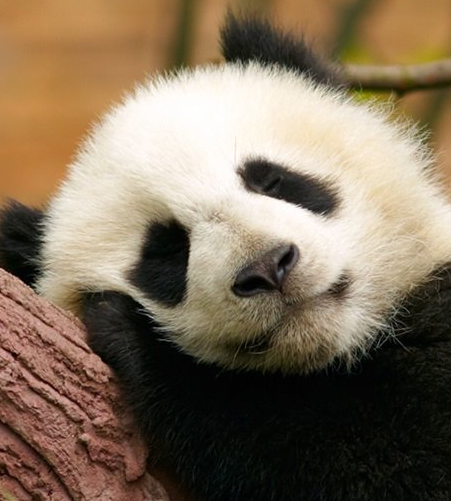
\includegraphics[width=0.6\columnwidth]{pandas}
\end{figure}
\begin{center}
{\Huge\CJKfamily{wxz}  铁憨憨}\\[1em]{\large\heiti 求职意向:数据分析师}
\end{center}

\cvsection{基本信息}
\begin{tabular}{@{}ll}
名族:& 汉\\
身高:& 180cm\\
体重:& 66kg\\
出生日期:& 1994.9\\
政治面貌:& 团员\\
\end{tabular}

\cvsection{联系方式}
\information{ \faPhone}{15511008888}\\
\information{\faEnvelope}{example@gmail.com}\\
\information{\faTwitter}{@example.com}\\
\information{\faMapMarker}{山西省西山县高老庄}\\
\information{\faGlobe}{\url{http://example.example.org/}}\\
\information{\faLinkedin}{\url{ http://www.linkedin.com/in}}

\cvsection{自我评价}

\hspace{2em}诸葛亮字孔明,琅邪阳都人也。汉司隶校尉诸葛丰后也。父圭,字君贡,汉末为太山都丞。亮早孤,从父玄为袁术所署豫章太守,玄将亮及亮弟均之官。会汉朝更选朱皓代玄。玄素与荆州牧刘表有旧,往依之。玄卒,亮躬耕陇亩,好为《梁父吟》。身高八尺,每自比于管仲、乐毅,时人莫之许也


\cvsection{编程技能}
\begin{center}
\progressbarr{python}{3+\,年}{60}

\progressbarr{\LaTeX}{3+\,年}{60}

\progressbarr{r语言}{5+\,年}{80}

\progressbarr{MATLAB}{5+\,年}{80}
\end{center}

\cvsection{编程技能}
\begin{center}
\progressbarr{python}{3+\,年}{60}

\progressbarr{\LaTeX}{3+\,年}{60}

\progressbarr{r语言}{5+\,年}{80}

\progressbarr{MATLAB}{5+\,年}{80}
\end{center}

\cvsection{编程技能}
\begin{center}
\progressbarr{python}{3+\,年}{60}

\progressbarr{\LaTeX}{3+\,年}{60}

\progressbarr{r语言}{5+\,年}{80}

\progressbarr{MATLAB}{5+\,年}{80}
\end{center}



\switchcolumn

\cvsection{教育背景}

\cvsbsection{2007.6-2009.9}{硕士学位 \quad 电子工程 }{清华大学}

\cvdetail{毕业论文:\kaishu 基于xxx对xxx的研究}

\cvdetail{主修课程: 数学分析,常微分方程,微分方程定性理论,高等代数,概率论与数理统计,近代概率论,实变函数与泛函分析,计算方法,算法分析等}

\cvdetail{blahblahblahblahblahblahblahblah}

\cvsbsection{2007.6-2009.9}{学士学位  \quad 信息科学 }{清华大学}

\cvdetail{毕业论文:\kaishu 基于xxx对xxx的研究}

\cvdetail{blahblahblahblahblahblahblahblah}

\cvdetail{blahblahblahblahblahblahblahblah}

\cvsection{科研项目}

\cvsbsection{2007.6-2009.9}{项目名称 }{}

\cvdetail{blahblahblahblahblahblahblahblah}

\cvdetail{blahblahblahblahblahblahblahblah}

\cvsbsection{2007.6-2009.9}{项目名称 }{}

\cvdetail{blahblahblahblahblahblahblahblah}

\cvdetail{blahblahblahblahblahblahblahblah}


\cvsection{工作经历}

\cvsbsection{2007.6-2009.9}{扫厕所}{中国石油化工集团公司}
\cvdetail{毕业论文:\kaishu 基于xxx对xxx的研究}

\cvdetail{blahblah}

\cvdetail{blahblah}

\cvsbsection{2007.6-2009.9}{刷盘子}{荷兰皇家壳牌石油公司}

\cvdetail{毕业论文:\kaishu 基于xxx对xxx的研究}

\cvdetail{blahblah}

\cvdetail{blahblah}

\cvsection{获奖\& 证书}
\cvprizedetail{2017.6}{“高教社杯”数学建模竞赛}{全国一等奖}

\cvprizedetail{2017.6}{“高教社杯”数学建模竞赛}{全国一等奖}

\cvprizedetail{2017.6}{“高教社杯”数学建模竞赛}{全国一等奖}


\cvprizedetail{2017.6}{“高教社杯”数学建模竞赛}{全国一等奖}

\cvprizedetail{2017.6}{“高教社杯”数学建模竞赛}{全国一等奖}

\cvprizedetail{2017.6}{“高教社杯”数学建模竞赛}{全国一等奖}

\cvsection{科研论文}

\smallskip
\hangindent=2em \hangafter=1
\wenxiannumber{1}\quad Carlo T.Takeo K.
Detection and Tracking of Point Features 
INTERNATIONAL JOURNAL OF COMPUTER VISION, 1991

\smallskip
\hangindent=2em \hangafter=1
\wenxiannumber{2}\quad Bill T.Philip M. Richard H. Andrew, F.Bundle Adjustment -- a Modern Synthesis 
VISION ALGORITHMS: THEORY AND PRACTICE LNCS, 2000

\smallskip
\hangindent=2em \hangafter=1
\wenxiannumber{3}\quad Carlo T.Takeo K.
Detection and Tracking of Point Features 
INTERNATIONAL JOURNAL OF COMPUTER VISION, 1991

\smallskip
\hangindent=2em \hangafter=1
\wenxiannumber{4}\quad David,C.
Inverse Acoustic and Electromagnetic Scattering Theory Second Edition 
1998

\end{paracol}
\end{document}
